\documentclass[tikz,border=5pt]{standalone}
\usepackage{amsmath}
\begin{document}
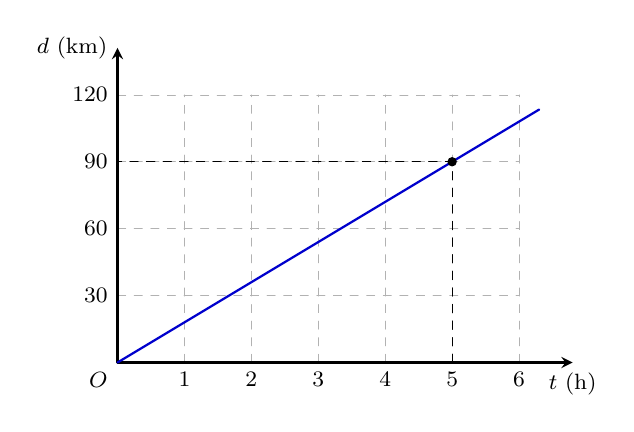
\begin{tikzpicture}[>=stealth, line join=round, line cap=round, font=\footnotesize, scale=0.85]
	\draw[dashed, black!30, very thin] (0, 0) grid (6, 4);
	\draw[->, thick] (0, 0) -- (6.8, 0) node[below] {$t\text{ (h)}$};
	\draw[->, thick] (0, 0) -- (0, 4.7) node[left] {$d\text{ (km)}$};
	\draw[thick, blue!80!black] (0, 0) -- (6.3, 3.78);
	\draw[dashed] (5, 0) -- (5, 3) -- (0, 3);
	\fill[black] (5, 3) circle (2pt);
	\foreach \x in {1,2,3,4,5,6} \node[below] at (\x, 0) {$\x$};
	\foreach \y/\v in {1/30, 2/60, 3/90, 4/120} \node[left] at (0, \y) {$\v$};
	\node[below left] at (0, 0) {$O$};
\end{tikzpicture}
\end{document}
